\chapter{Technik/Methoden}
\label{cha:Technik}

\section{Das Kühlregal}
\label{sec:Das Kühlregal}

Der Mittelpunkt der durchgeführten Untersuchungen ist ein Kühlregal der Firma AHT.
Es umfasst auf einer Länge von \unit{3,75}{\metre} vier Regalböden um Produkte zu kühlen und auszustellen. Ein von oben herabfallender Luftschleier ermöglicht ein türloses Design des Regals. Die Kälteerzeugung wird, wie in Abbildung~\ref{fig:IDC150} ersichtlich, durch drei seperate Kältekreisläufe gewährleistet. Das verwendete Kältemittel ist Propan (R290). Jeder Kreis besitzt eine Füllmenge von \unit{150}{\gram}. Um die Füllmenge zu reduzieren wurden bereits vor Beginn der Untersuchungen kältetechnische Komponenten mit geringerem internen Volumen eingebaut. Die Verdichter sind ein Produkt der Firma Emerson. Im Rahmen der Untersuchungen kommen mehrere Modelle zum Einsatz. Drei Plattenwärmeübertrager der Firma SWEP dienen als Verflüssiger. Sie besitzen je 20 Platten und eine Nennleistung von je \unit{2,7}{\kilo\watt}. Die Expansionsventile der Firma Alco sind elektronisch regelbar und besitzen einen Temperatur- sowie Drucksensor in der Saugleitung. Die drei Kreisläufe durchlaufen mit je sechs Durchgängen einen gemeinsamen Verdampfer dessen Lamellenabstand \unit{5}{\milli\metre} beträgt. Sechs Lüftermotoren der Firma EBM Pabst saugen die Luft durch den Verdampfer mit einer konstanten Drehzahl von \unit{1400}{U\per\min}.

\begin{figure} %[!htb]
\centering
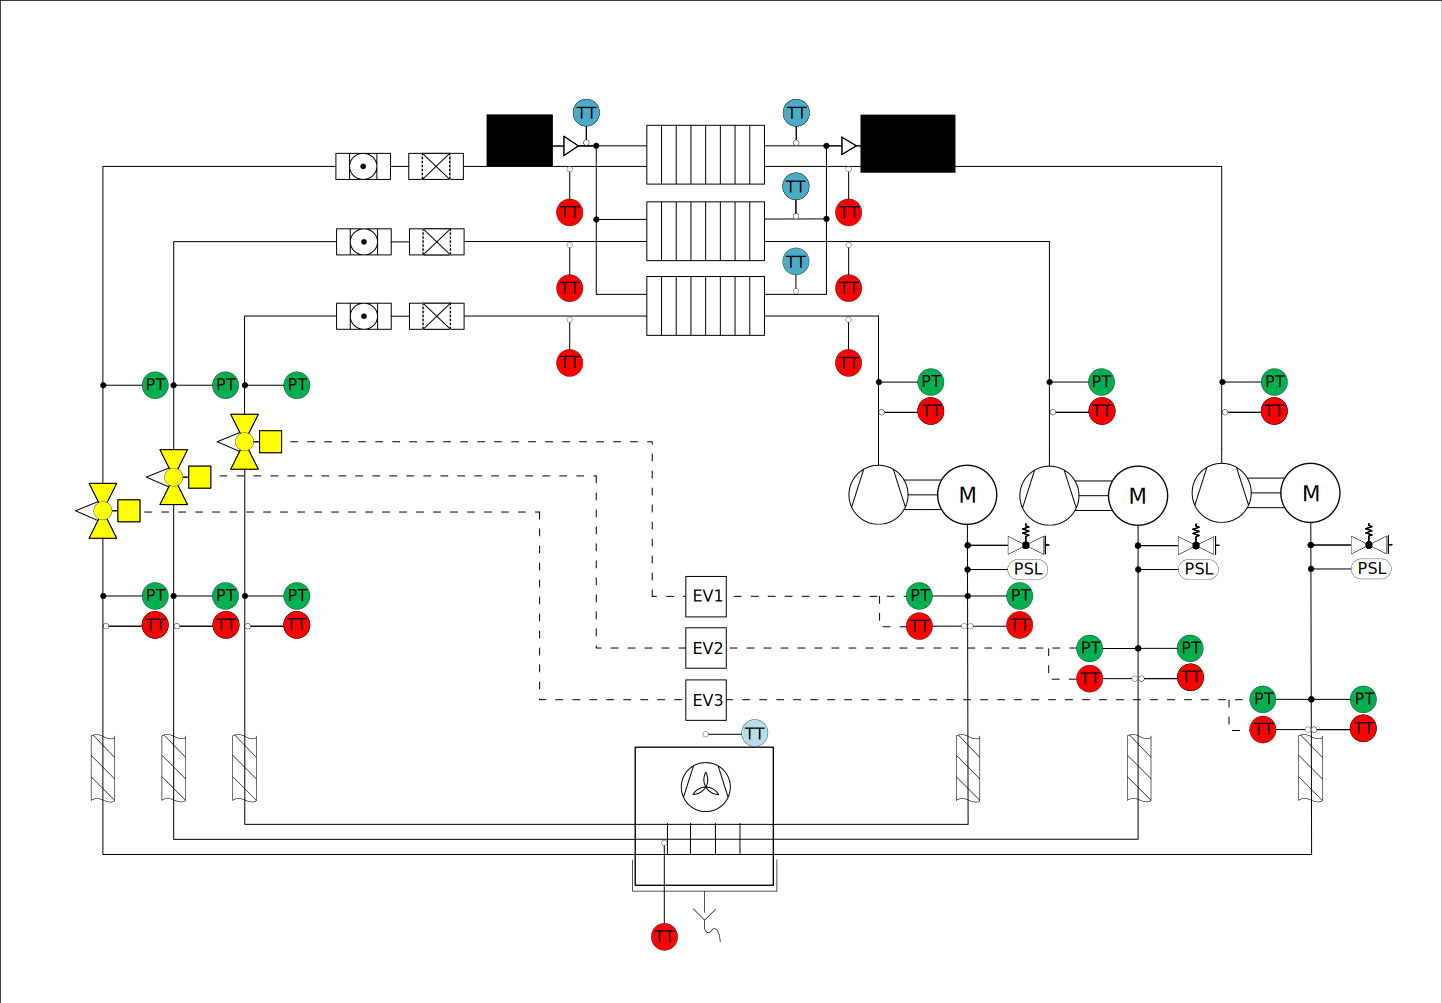
\includegraphics[scale=.5,angle=90]{Pictures/IDC150.pdf}
\caption{IDC150}
\label{fig:IDC150}
\end{figure}


\section{Die Klimakammer}
\label{sec:Die Klimakammer}

Um während den Untersuchungen gleichbleibende Umgebungsbedingungen zu generieren und so reproduzierbare Ergebnisse zu erzielen, steht das Kühlregal in einer Klimakammer.
Wie in Abbildung~\ref{fig:Klimakammer} zu erkennen besteht die Klimakammer eigentlich aus zwei kleineren Kammern mit eigenständigen Zuluftregelungen. Aufgrund der Größe des Regals wurde die Trennwand zwischen den Kammern entfernt. Die Zuluftaufbereitung übernimmt dabei die Klimaanlage der Kammer B. Damit die aufbereitete Luft den Raum über seine gesamte Länge durchströmt wurde die Ansaugöffnung von Kammer B mit einer Decke, die bis zum Ende des Raums reicht, abgedeckt. Vor den Luftauslassgittern besitzen die Kammern Umlenkbleche. Diese sollen eine gleichmäßige Verteilung des Luftmassenstroms über den Austrittquerschnitt erzielen. Die Klimaanlagen sind in der Lage die angesaugte Raumluft zu kühlen, aufzuheizen, sowie zu be- und entfeuchten. Die Regelung findet dabei über einen Computer statt. Mithilfe von LabView, welches eine intuitive Benutzeroberfläche bietet, lässt sich Einfluss auf die Soll-Werte, die Dauer der jeweiligen Untersuchung und die Einstellung der Regelparameter nehmen. 
Jede Kammer besitzt zudem einen Wasseranschluss dessen Vorlauftemperatur regulierbar ist.
Die Verflüssiger des Kühlregals werden mit temperiertem Wasser der Regelung von Kammer A beaufschlagt. 


\begin{figure}[htb]
\centering
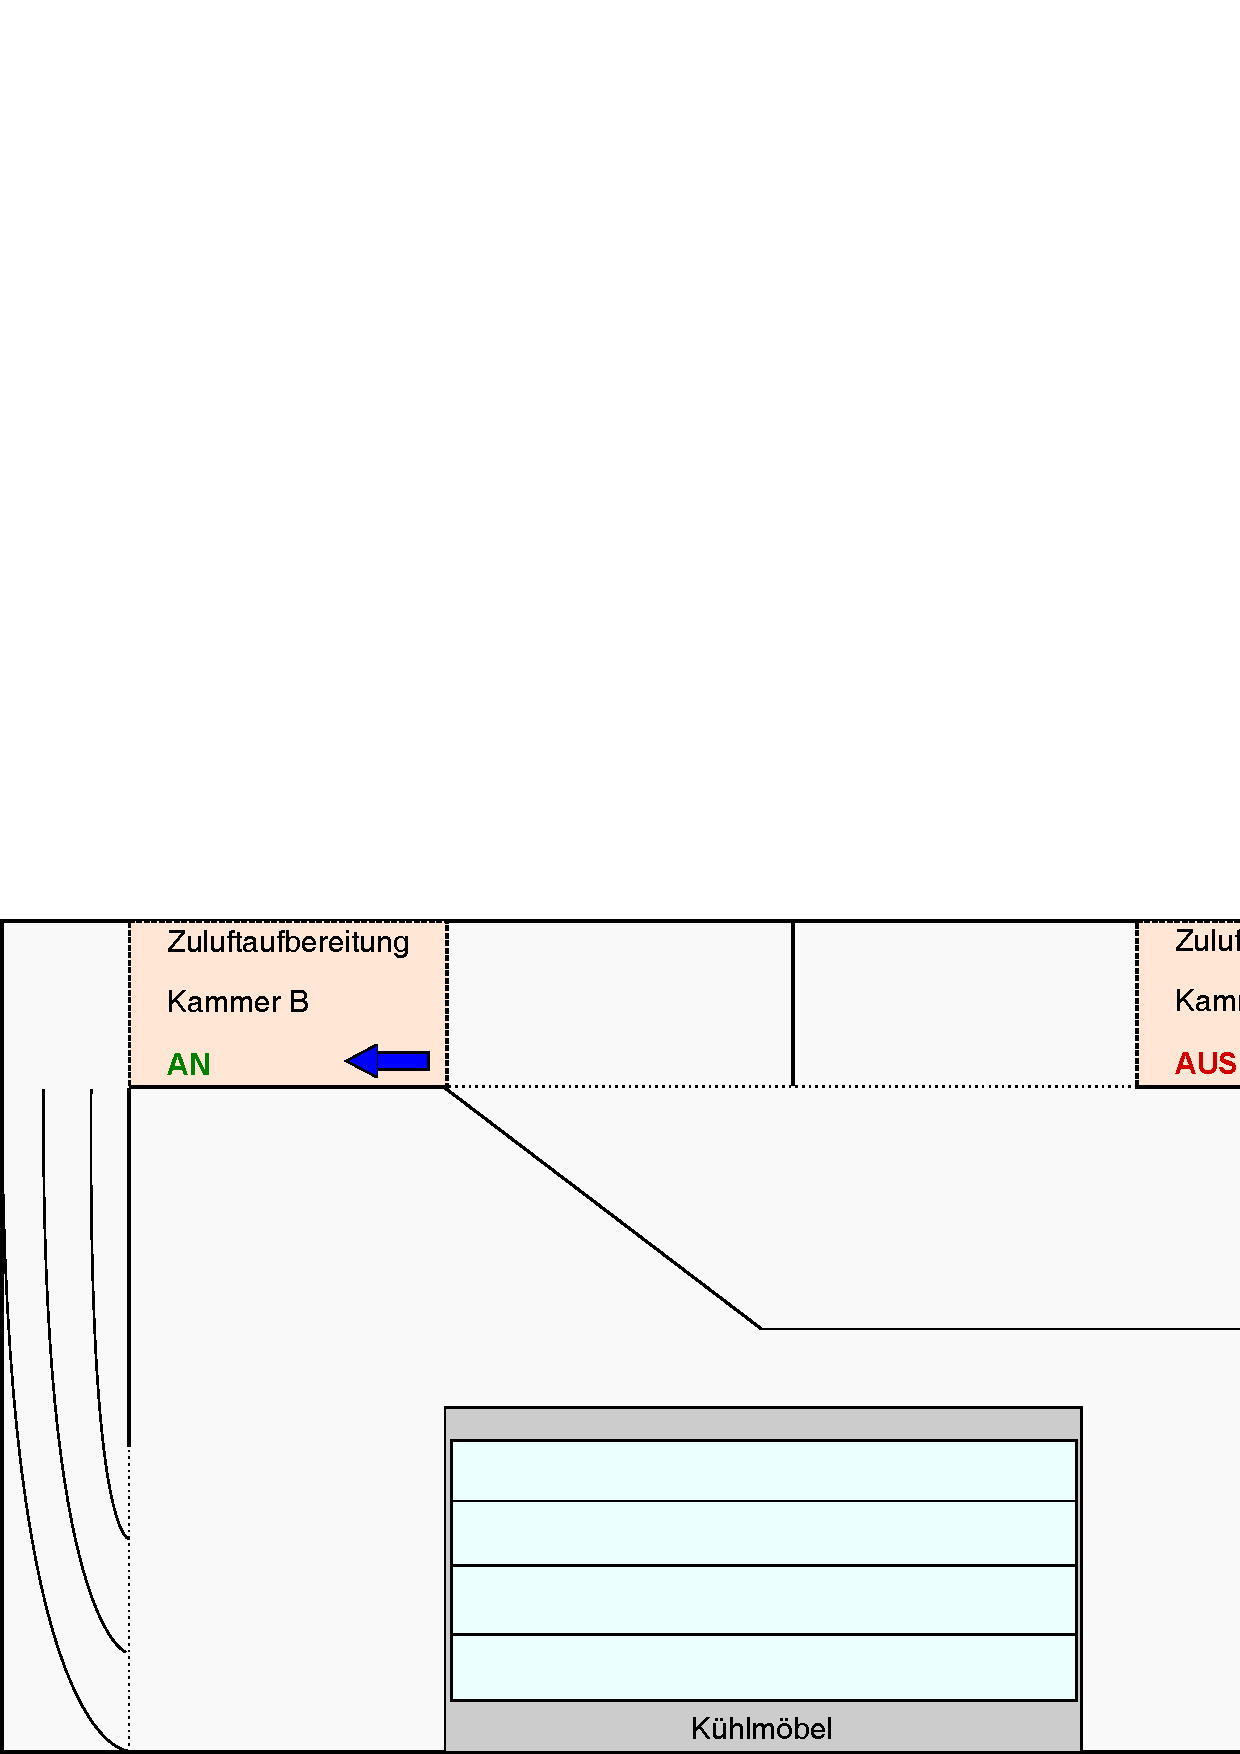
\includegraphics[scale=.5]{Pictures/ClimateChamber.pdf}
\caption{Klimakammer}
\label{fig:Klimakammer}
\end{figure}

\section{Erfassung von Messdaten}
\label{sec:Erfassung von Messdaten}

Um alle physikalischen Größen während des Betriebs möglichst genau zu erfassen und zu speichern werden entsprechende Geräte und Programme eingesetzt. Insgesamt finden drei Systeme Anwendung um sensorbasiert Daten zu erfassen, umzuwandeln und in Tabellenform zu speichern.

\subsection{Messdaten der Klimakammer}
\label{subsec:Messdaten der Klimakammer}

Die in Abschnitt~\ref{sec:Die Klimakammer} vorgestellte Klimakammer wird über LabView gesteuert. Die erfassten Messdaten sind raumluftseitig Ist- und Mittelwerte der Temperaturen sowie die relative Luftfeuchtigkeit. Wasserseitig werden Wassermassenstrom sowie Vor- und Rücklauftemperatur gemessen. 
Die Sensoren, welche die Regelgrößen Temperatur und relative Luftfeuchtigkeit aufnehmen, sind zuluftseitig in der Nähe des Auslassgitters positioniert. Die Regelgröße der Temperatur entspricht dem Mittelwert von drei, über die Höhe des Luftauslassgitters verteilten Temperatursensoren. Wird der Betrieb der Klimakammer über das Programm gestartet so wird eine Exceldatei erstellt in die in einem Intervall von \unit{1}{\second} die erfassten Daten geschrieben werden.


\subsection{Messdaten des Kühlregals}
\label{subsec:Messdaten der Klimakammer}

Mithilfe des Programms NI SignalExpress werden die Messdaten des Kühlregals und der Kältekreisläufe via Modbus erfasst. Um die Temperaturen zu messen werden Thermoelemente  und um die Drücke zu messen Hochgenauigkeitsdruckaufnehmer verwendet. Die erfassten Messwerte sind die Produkttemperaturen sowie Ein- und Austrittstemperatur der Luft am Verdampfer des Kühlregals, die Temperaturen an verschiedenen Positionen der Kältekreisläufe und die Relativdrücke des Kältemittels im System in Heißgasleitung, Flüssigkeitsleitung, Einspritzleitung und Saugleitung. Die Positionen der Sensoren an den Kältekreisläufen sind aus Abbildung~\ref{fig:IDC150} ersichtlich. Zudem wurde noch die Temperatur des Kältemittels nach jedem einzelnen Durchgang durch den Verdampfer erfasst.
In einem Intervall von \unit{5}{\second} werden die erfassten Daten in eine Exceltabelle geschrieben. SignalExpress erstellt in Echtzeit Graphen der Messwerte. Somit lässt sich das Verhalten des Systems jederzeit beobachten.

\subsection{Messdaten des Leistungsanalysators}
\label{subsec:Messdaten des Leistungsanalysators}

Um den Zustand des Systems auch elektroseitig zu erfassen wird ein Yokogawa WT3000 Leistungsanalysator verwendet. Dieser ist in der Lage Spannungen, Ströme mit einer Genauigkeit von \unit{0,02}{\%} zu erfassen und daraus Blind-, Wirk- und Scheinleistungen zu berechnen. Die abgenommenen Komponenten sind die einzelnen Verdichter, die Ventilatoren und die restlichen Verbraucher des Kühlregals, wie Licht und Relays.
Das Gerät speichert die erfassten und berechneten Messwerte in Tabellenform auf einem externen Datenspeicher. Die Intevalllänge beträgt hierbei \unit{5}{\second}.


\section{Testbedingungen nach Norm}
\label{sec:Testbedingungen nach Norm}



\chapter{Prüfstand}
\label{cha:Prüfstand}





%\begin{figure}[h]
%   \centering
%   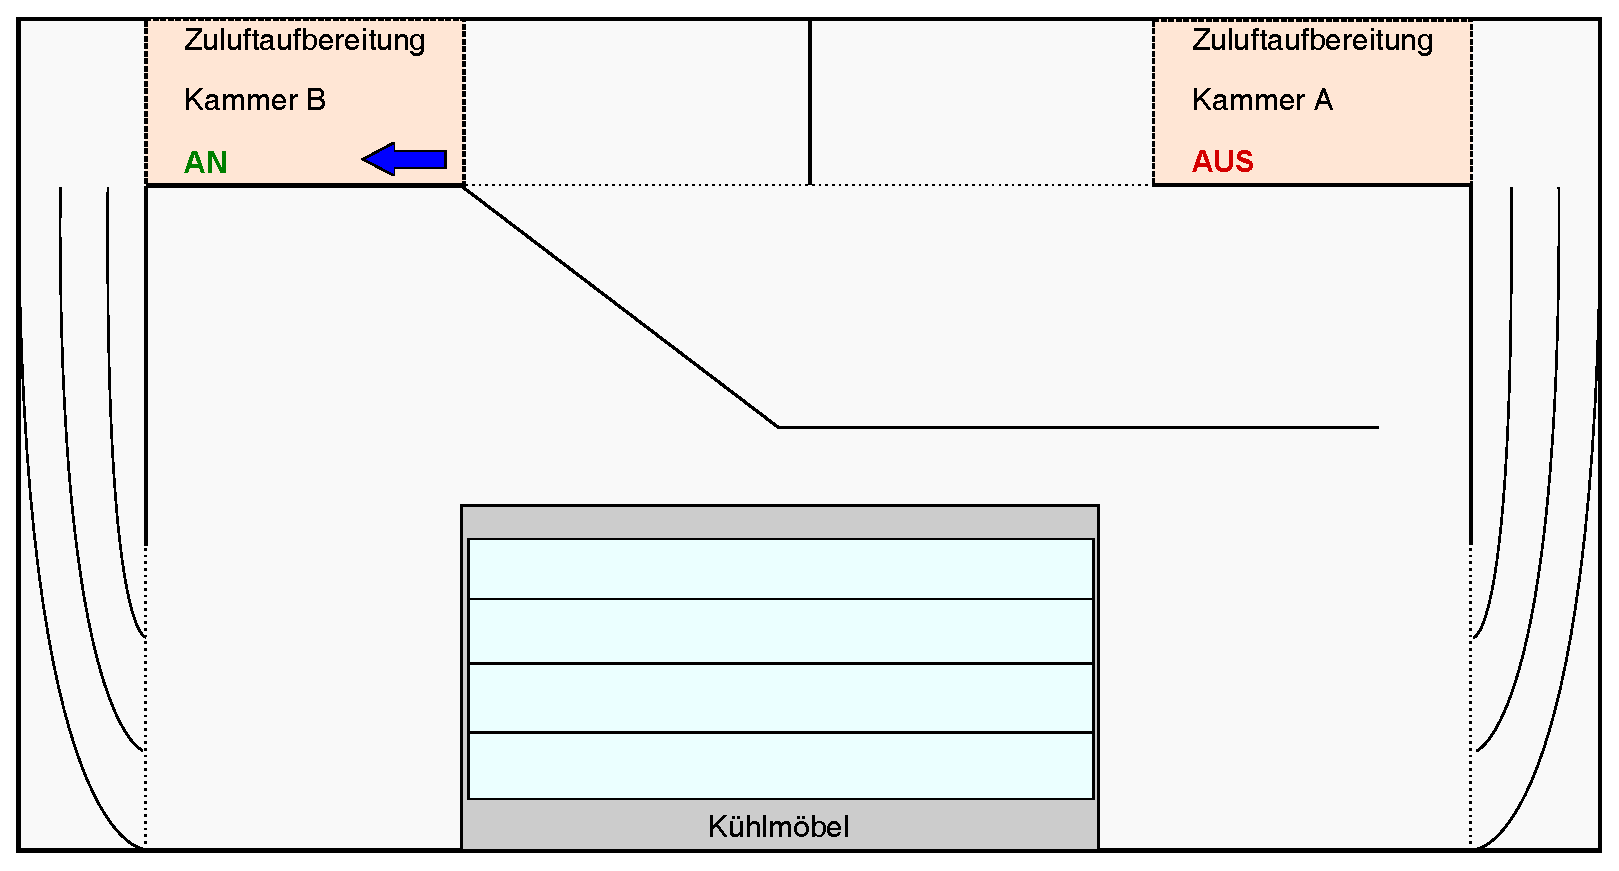
\includegraphics{Pictures/ClimateChamber.eps}
%\end{figure}

Grafiken:
Klimakammer Inkscape
Quellen:
DIN EN ISO 23953